\documentclass[11pt]{article}
\usepackage[utf8]{inputenc}
\usepackage{fullpage}
\usepackage{hyperref}
\hypersetup{colorlinks=true, linkcolor=blue, filecolor=magenta, urlcolor=blue, pdftitle={Group 48 Final Report}}
\usepackage[skip=8pt plus1pt, indent=0pt]{parskip}
\usepackage{graphicx}

\newcommand{\codeword}[1]{\texttt{#1}}

\begin{document}

\title{Group 48 Final Report}
\author{Bingqi Li \and Haoran Wang \and Leven Zhou \and Zhanrong Qiao}

\maketitle

\section{Assembler}

During the development of the assembler, we explored several data structures to best support different requirements.

\subsection{Symbol Table}

Initially, the symbol table was implemented as a singly linked list, storing label-address pairs in each node. This structure has $O(sn)$ search complexity using the linear search algorithm to stop at the node with corresponding label, where $n$ is the number of labels and $s$ is the length of each label. Recognising this as a rather slow approach, an improvement was scheduled to convert the symbol table to a BST, reducing the complexity to $O(s \log n)$. However, after a brief discussion within the group, we decided to use a simpler, and probably even faster approach: \textit{tries}. In this way, insertions and searches both have $O(s)$ complexity, the same as a hash table. Compared to a hash table, a trie uses less memory, and is slightly simpler to implement since we do not need to handle hash collisions (\textit{linear probing} has the risk of severe performance degradation when the table is almost full, and \textit{separate chaining} still requires linked lists).

\subsection{Structure}

As for the assembling process, the initial strategy was parsing the whole file into some data structure and then doing the assembling using information stored in that structure. But whenever we want to support a new syntax, the structure has to be modified to hold more information; being just an alternative representation of the file content, it looked redundant after some time. It turned out that we could do without it, by re-organising the process into a kind of ‘syntax-directed’ translation (parsing the file and generating instructions at the same time). In order to implement our idea, we developed different kinds of ‘tokens’ to support various types of information in the file, like comma, hash sign, immediate value, etc. and a ‘tokenizer’ which converted the input file content to a series of tokens so that we could process token by token to generate the corresponding instruction. With the help of the upgraded parsing strategy, the code became more coherent and logical, and adapting to new syntax became easier.

\section{Extension}

We extended the emulator and assembler to support more instructions (those used in function calls, including \codeword{PUSH}, \codeword{POP}, \codeword{BL} and \codeword{BX}), and enabled the emulator to dump a part of its memory as a bitmap file (so that we could have graphical output from the emulator). We then used Zhanrong’s side project, an interpreter for a Scheme-like language, to implement a compiler that could turn a tiny subset of C into the subset of ARM assembly supported by our emulator. With its help, we were able to build a simple ray tracer that runs on our emulator. Finally, Haoran (the only Computing student in our group) implemented a post-processing filter that adds to the bitmap output some artistic quality. This was done in standard C.

\subsection{Example of Use}

In the \codeword{src} directory, execute \codeword{make release} to build the assembler, emulator and ‘wirenizer’ (a standalone program of the post-processing filter).

To build the ray tracer, you will need to \href{https://github.com/bridgekat/apimu/releases/tag/v0.1-alpha}{download} the executable file of the Scheme interpreter (for platforms other than Linux x64, you will have to \href{https://github.com/bridgekat/apimu#building-experimental}{build from source}). Then, place the \codeword{testeval} executable in the \codeword{extension} directory, and execute \codeword{make} there. This will generate \codeword{raytracer.out}.

To use the wirenizer filter, type \codeword{./wirenizer <input-filename> <output-filename>}. Currently, only 24-bit (true colour) BMP files are supported.

To run the ray tracer, change directory to \codeword{extension}, type \codeword{../src/emulate raytracer.out <memory-size> <stack-size> <framebuffer-width> <framebuffer-height> <output-filename>} or directly execute \codeword{./run.sh}. The output file will be a 24-bit (true colour) BMP file.

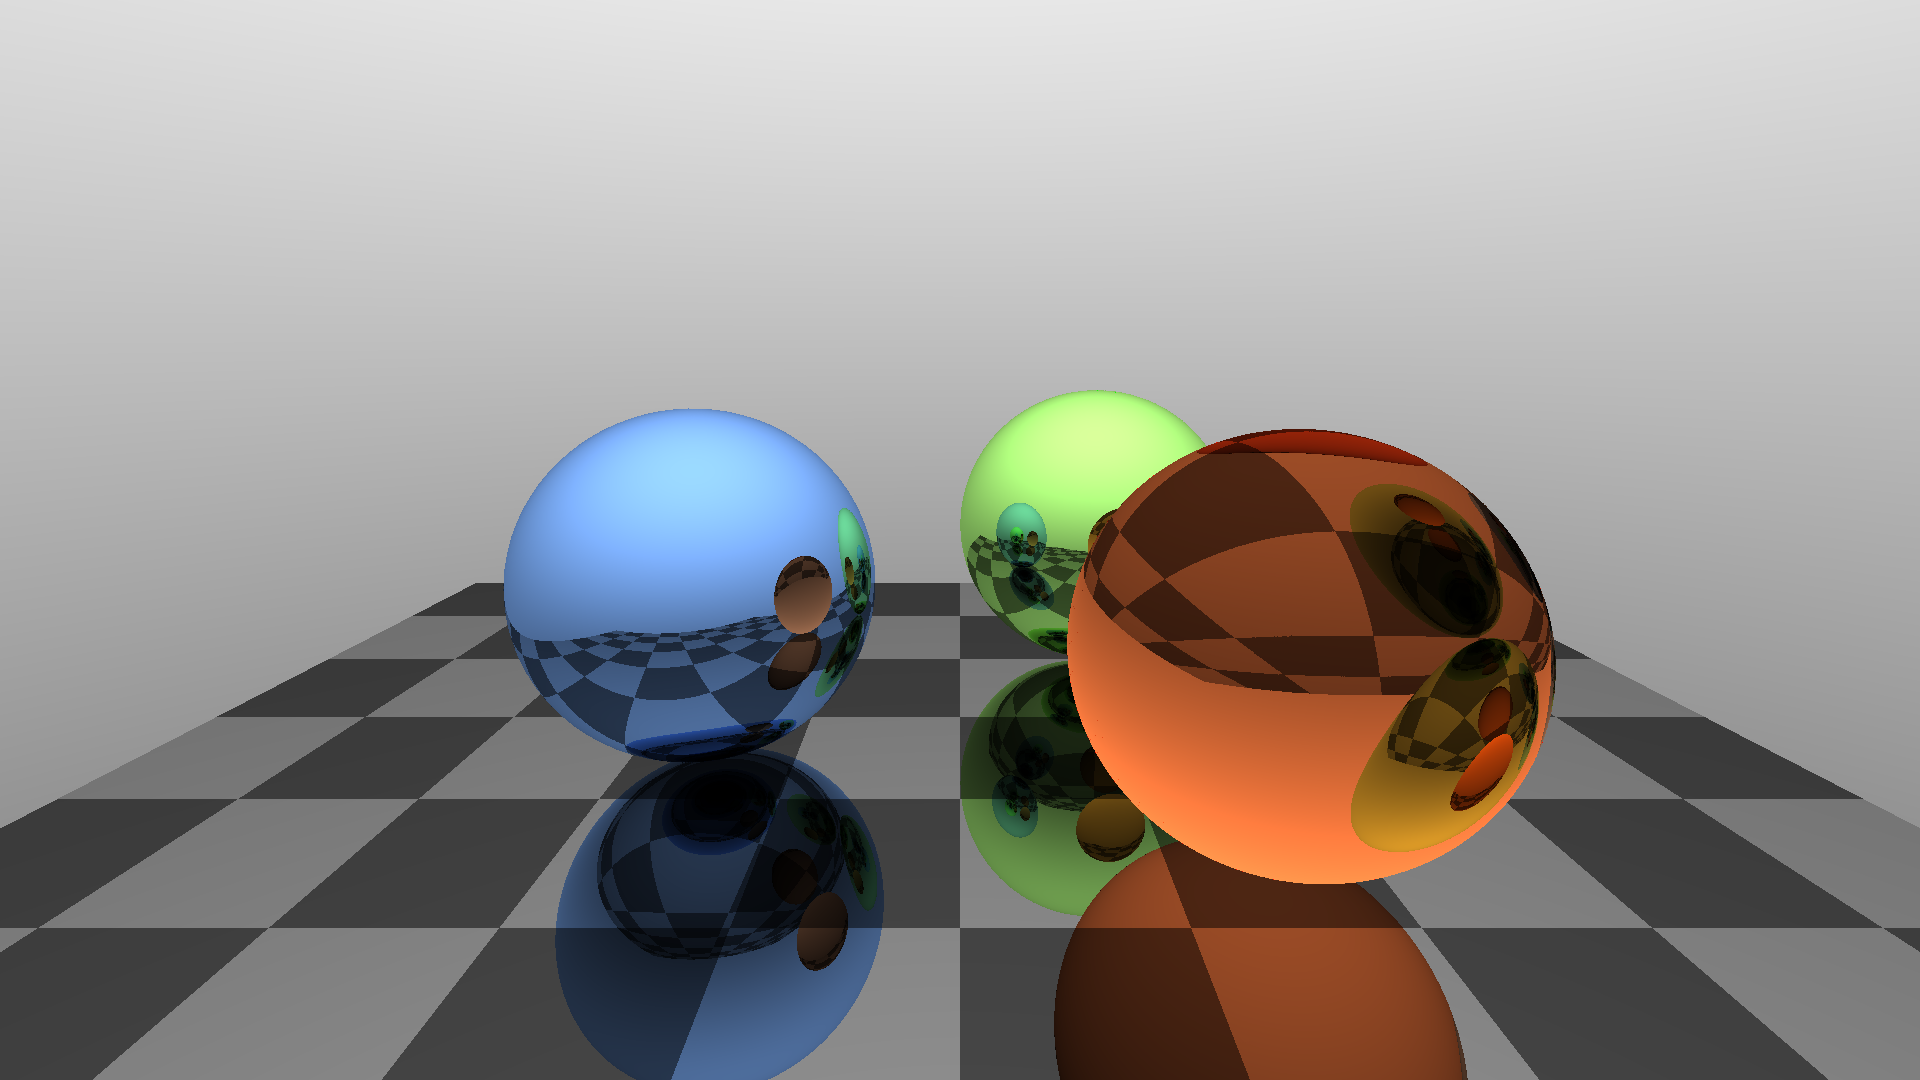
\includegraphics[width=.49\textwidth]{images/output.png}
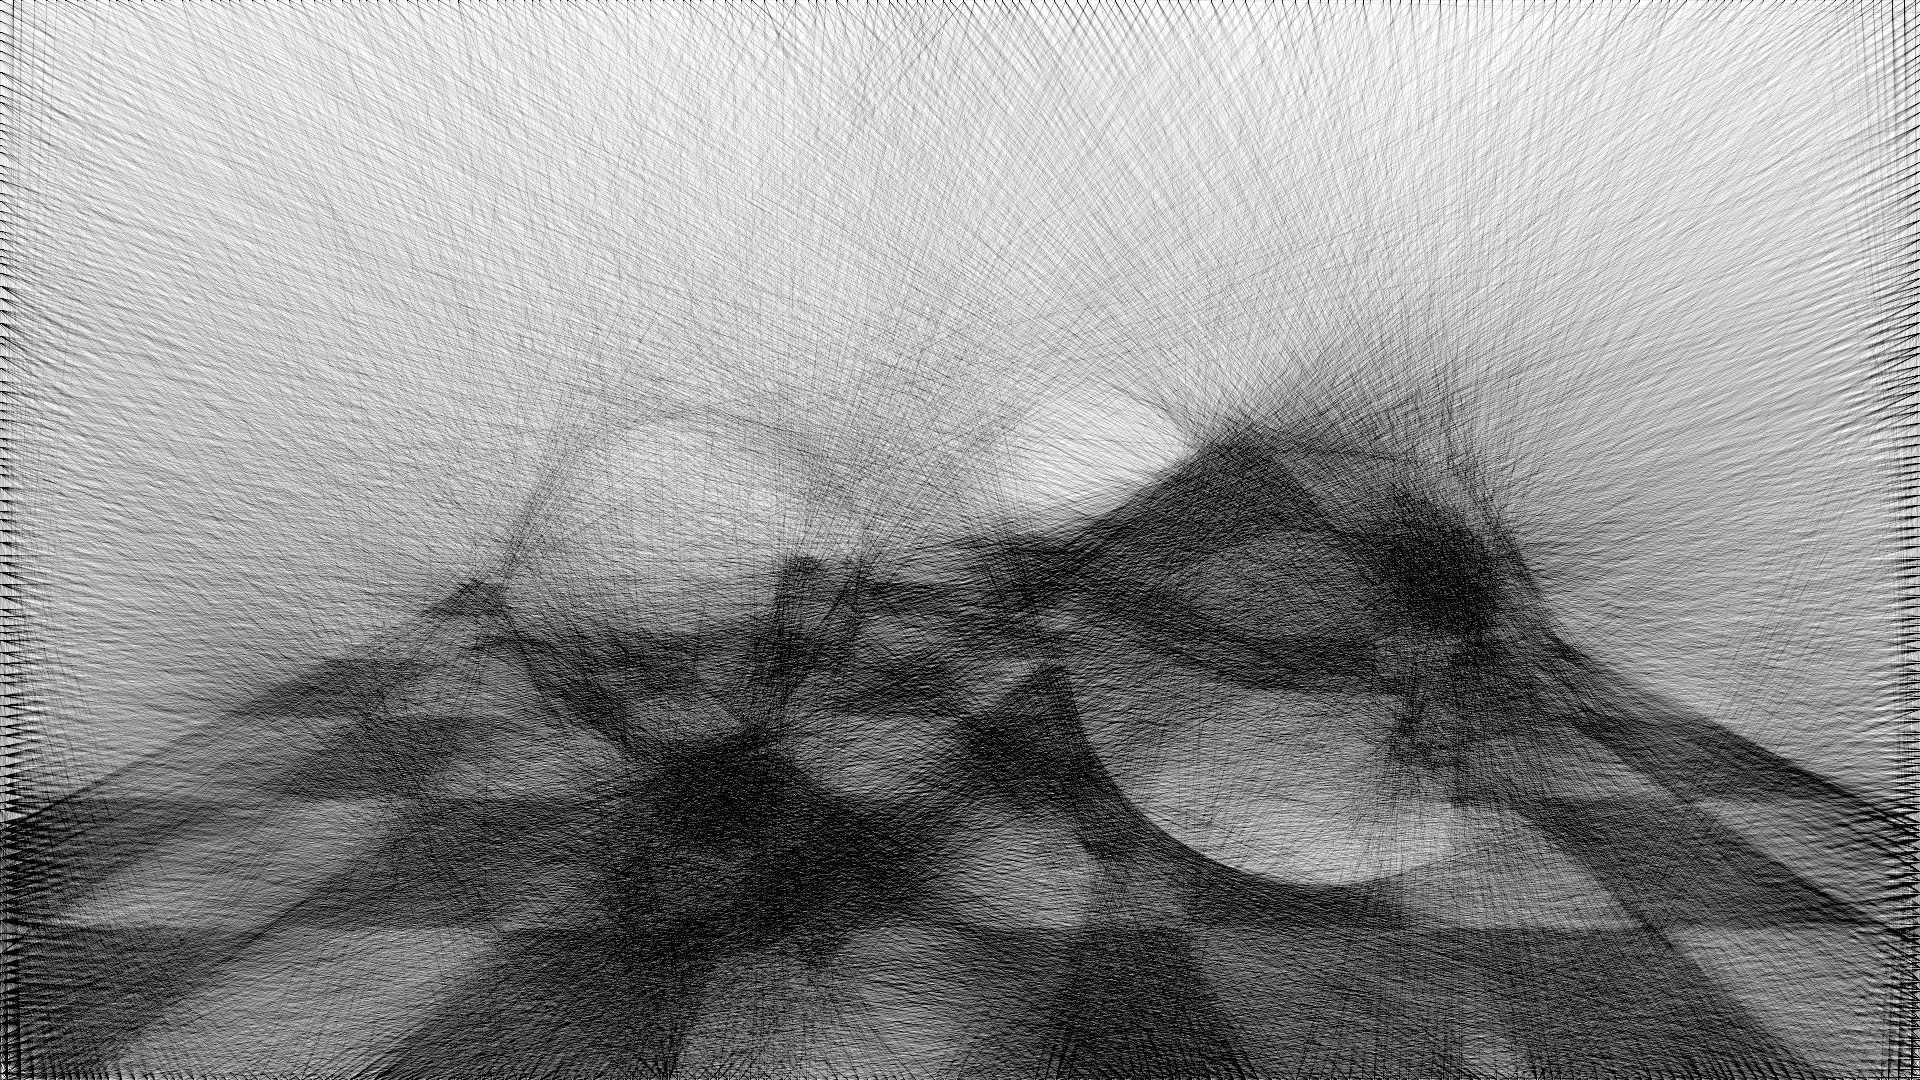
\includegraphics[width=.49\textwidth]{images/post.png}

\subsection{Design}

Our code structure of the emulator and the assembler makes it easy to extend them with new instructions. The parser code is very modular, and is able to parse LL(k) grammars easily. We could actually reuse it to write the compiler, but Zhanrong considered his variant of Scheme to be an even better choice. It has an \href{https://en.wikipedia.org/wiki/Earley_parser}{Earley parser}, capable of parsing arbitrary context-free grammars, and allows the user to \href{https://github.com/bridgekat/apimu/blob/main/scripts/prelude.mu}{reconfigure its syntax} (like the \codeword{\#define} directive in C, with the power of redefining everything). We could embed a language in it with relatively little boilerplate code, and writing compilers in a functional language probably reduces the amount of boilerplate too. Moreover, this would give Zhanrong a chance to find problems in his Scheme interpreter and improve it. Finally, Zhanrong has never written a compiler back-end before, and he had no idea on how to compile higher-order functions and first-class continuations. This prevented him from writing a compiler for the Scheme itself; a subset of C seemed to be much more doable.

We implemented just enough features in the emulator, assembler and compiler to support the implementation of a simple ray tracer \textit{(more details can be found in our slides)}. For example, we did everything with fixed-point numbers so that we don’t need to implement a heap of floating-point operations in the emulator. This also has the advantage that if other students ever wanted to try running it on their emulator, they only need to implement a minimal number of additional features.

We are not sure if such an extension is considered legitimate, since it was \textit{not} written in standard C. But Haoran’s filter definitely was. It turns a coloured picture into a cluster of lines while preserving the overall composition of the picture. The algorithm: specify a set of points, for each pair of points calculate the average brightness of the pixels on the line segment connecting them, choose the darkest line segment, add it to the result set, and brighten the line segment on the picture. Repeat the process until the picture is sufficiently bright. The resulting set of lines forms another picture that resembles the original one, but more artistic…

\subsection{Challenges and Problems}

\subsubsection{Compiler}

In implementing the compiler, we simply translated every sub-expression of a program to assembly code (or more precisely, a kind of low-level linear IR) recursively, and as a convention, every piece of translated code stores its final result in register 0 (whenever applicable). The code of a binary operation node, for example, was obtained by ‘merging’ that of its two child nodes, appended by a new instruction calculating the end result from LHS and RHS. The code for ‘if’ and ‘while’ nodes is similarly recursively defined – using conditional branches and labels.

The biggest challenge was probably about register allocation. The first version simply juggled between two registers, one for LHS and the other for RHS, pushing and popping intermediate results in each ‘merging’ operation. Looking at the generated assembly, we found that many stack operations were clearly redundant. Later, we used a slightly improved method: keep track of the registers used by each piece of generated code, and, when merging two pieces of code, rename all registers in the second piece so that \textbf{it will not affect the value of register 0} and \textbf{will store its end result in register 1}. Only when such renaming is impossible would we use the stack to store the intermediate result from the first piece. This eliminated a lot of redundant pushes and pops.

The introduction of function calls made things even more complicated. The standard calling convention in ARM architectures allows registers 0-3 to be modified by a function call, but all functions must preserve the values of registers 4-11. The former requirement made our naive renaming approach much less effective. So we ‘invented’ a non-standard protocol to simplify the problem: every function must save its return value in register 0 (if applicable), but also preserve the values of register 1-11. Then we changed the default register to store intermediate results from r0 to r1. A true solution will likely involve static single-assignment form and graph colouring, which we had not enough time to implement…

\subsubsection{Ray Tracer}

Since we didn’t have floating-points, we wrote fixed-point arithmetic instead. Our fixed-point representation consisted of a sign bit, 15 bits of integer part and 16 bits of fractional part. The initial method of doing multiplication simply shifted two operands to the right by 8 bits and did a normal multiplication. This is acceptable if both operands have roughly the same magnitude, but if one of them is large and one of them is small, the smaller one will lose more relative precision. As a result, the quality of the generated image was poor. We then tried splitting both operands into the lower 8 bits and higher 24 bits, and doing three multiplications: higher times higher, lower times higher, and higher times lower (we didn’t do lower times lower, as the result never exceeds epsilon, and we didn’t care that much about correct rounding). This provided a much better result.

Another problem was caused by the compiler: it does absolutely no optimisation. All local variables are ‘physical’, and every read/write to them translates into several memory-accessing instructions. This is clearly not suitable for some performance-critical parts of a ray tracer. So we wrote them (fixed-point arithmetic and vector operations) in assembly.

We also had to implement common mathematical functions (inverse, sine, cosine and square root) by ourselves. These were done by Newton’s method and Taylor expansions. To avoid divergence or degradation of precision, we need to normalise the input before actually applying the algorithms.

Finally, the spec says when we \codeword{LDR} a constant into a register, we need to put that constant at the end of the assembled program and load it from there. But as the generated assembly grew to more than 1024 instructions, the offset might exceed 4095 – the maximum number representable in 12 bits. We need to make space at some place nearer to this instruction to store the value. Since doing so changes the addresses of some labels, it must be implemented as an intermediate pass. This was a niche problem anyway, so we did not implement a solution, but instead avoided writing constants not representable as an ‘immediate value’ in our ray tracer program. If some were indeed unavoidable, we put that procedure near the end of the program so that no offset exceeded 4095.

\subsubsection{‘Wirenize’ Filter}

Some problems arose during the first implementation of the \codeword{buildCircle} function. For generating points on a circle, the original idea was to traverse every pixel of the picture and calculate its distance to the centre, selecting those whose distance are exactly the same with radius. But then, only a few irregularly distributed points were generated. The main reason of the problem was that we only considered the ‘grid points’, and the condition that radius equals distance exactly was rarely met. With a discussion within the group, we changed the strategy into traversing the circle and finding all the possible positions of points by using sines and cosines. Although most of them would not exactly land on a ‘grid point' (coordinates are not integers), they were rounded to the nearest one. In this way, the problem of uneven distribution of points was solved.

\section{Reflection}

\subsection{Group Reflection}

Before we started coding, we learned to use Git under a collaborative setting, which involves merging conflicts, branching and rebasing. From there we went down smoothly – we finished the emulator in four days, assembler in one week, compiler and ray tracer in about one week, and the post-processing filter in two days. It was already beyond our expectations.

% During the project, we’ve also found it important to build reusable functions for recurring patterns. Decoding instructions, for example, involves repeatedly taking bits from an unsigned integer. At first, these were all done by direct bit manipulation. There were lots of magic numbers; for readability, we had to write comments that indicate \textit{which} bits we were taking. Even with these comments, we still found errors in each other’s code. Then it turned out that all these could have been implemented as a one-line helper function. The arguments to the function themselves indicated the bits we were taking, so there was no need for extra comments, and errors could be prevented with relative ease.

In future projects, we will continue to try different ways to structure the code, and aim for better efficiency and less redundancy. We will try to make everything simple and extensible. We will continue to review each other’s code to ensure correctness.

\subsection{Individual Reflections}

\subsubsection{Bingqi Li}

This is the first time I have participated in a group programming project. It was a unique and rewarding experience overall. Instead of having to concern about the entire codebase all by myself as I did in all of my past personal projects, I learned to collaborate with groupmates through communication, taking share of the responsibility and interacting on others’ products with trust (peer code review still takes place to reinforce correctness, of course). Learning more advanced git operations (\codeword{pull}, \codeword{merge}, etc) also proved to be useful in making the development process run smoothly, which can also be applied in all future group projects. Surely being part of a group project does not mean to depend on groupmates completely, taking my own initiatives was equally as important. During the development of the assembler, I volunteered to lay out the skeleton and implement the control flow, taking into consideration how it may be based on and interacted with to support more precise functionality to be implemented in the future. Through frequent meetings and discussions, the assembler improves and grows into such shape that all of us are proud of. This gives me a strong impression on how developers can collaborate towards completing a big project that can be otherwise difficult to achieve individually. The skills obtained in the process are truly invaluable.

\subsubsection{Haoran Wang}

I have never participated in a group programming project before. This experience was totally fresh and unforgettable to me. I have witnessed the progress of building such an enormous project from template by breaking it down into smaller separate pieces and tasks assigned to each group member. We can’t accomplish such a big project without everyone’s contributions. During the frequent discussions within the team, I have learned to spill out any ideas and suggestions bravely on others’ implementations, and accept others’ superior implementation strategy and code structures with an open mind. Designing a reusable and extendable data structure when building the template of a project really matters. It turns out to avoid implementing redundant functionally similar structures for particular functionality and save a lot of time. This will provide me with alternative ideas and scopes on structure designing in the future. Keeping enthusiasm and initiatives on researching fields I am not familiar with is also important. In the exploration of extensions, all my ideas at first were proved to be infeasible due to lack of information and limited amount of time during the halfway, I have to remove those partially implemented functions and start anew which frustrated me. But continuously reading useful information finally inspired me and I finished my own extension part. When I saw the final successful running results of the extended functionality, I realised how significant it is to keep consistent and initiative. Overall, the treasuable experiences I learned in the project and team work really enlightened me. I am glad to have such a chance to work with my excellent teammates.

\subsubsection{Leven Zhou}

I did not contribute a lot to this project since I got sick when starting the C course and failed to catch up after the project had already started. Zhanrong completed the skeleton frame of the project very soon and left some functions to the rest of the group members. I was quite confused in the first place since I just started to watch the C lectures. Zhanrong explained to me and with his help, I finished the function I was assigned to. When I felt better later, I hurried to finish the C course. However, the assembler part was also almost finished at that moment. I read and tried to understand the code they wrote, luckily I learned a lot from doing these and got great progress in C. Then I fixed some errors, debugged one of the functions and optimised some of the code. This is the first time I have participated in a group programming project. It is definitely a whole new experience and I am able to learn from others’ coding style and methods. As I said above, my teammate helped me a lot and did most of the project because of my physical condition, I am not a good teammate to them. I will learn from this experience and be more proficient in programming, and do better in future’s group projects..

\subsubsection{Zhanrong Qiao}

This is definitely \textit{not} the first time I have participated in a group programming project. But it is the first time I have participated in an \textit{assessed} one. The biggest difference is that everyone is expected to learn something from it – simply completing the task is not sufficient alone for a good score, without for example a good distribution of work. I made a boilerplate for the emulator as a reference, proposed to let everyone implement a part of the instruction handlers (the cores of our emulator/assembler), and other data structures they see fit; and explained the use of Git under a collaborative setting, since many of us probably had little such experiences before. I have also undertaken code review to ensure the correctness of our code, sometimes making radical changes for a better structure. I was amazed to see that some of us (especially Bingqi) could already produce quality code in their first months of C experience! And I was glad that they all understood my proposals with just a little explanation.

However, with almost eight years of experience in C++ and algorithms, I sometimes felt overly confident and took other people’s responsibility, or forgot to leave work for them when trying to implement new features. I also tend to disregard the spec while doing the extension (none of what I have proposed and done was in standard C), leaving Haoran having to find a better way out by himself (he had to come up with the idea and initial implementation, though I provided some help later.) My excuse would be that this project is worth only 5-8\% of a module, so I did not pay attention to every detail; but I could probably try to do better next time. \footnote{Finally, due to my shyness and unfamiliarity of living in a foreign land, I have relied heavily on Bingqi in collecting housing information and looking for accommodation for next year. While I was experimenting with the compiler stuff, Bingqi (apart from making significant direct contributions to the emulator and assembler) was putting lots of effort in contacting landlords and finally found a place for me, saving me a lot of time and from potential troubles. In regard to this, he probably made the most contribution to the progress of our project…}

\end{document}
